%% -*- Lecture -*-

\synctex=1
\documentclass[11pt]{beamer}
\usepackage{microtype}
\usepackage[utf8]{inputenc}
\usepackage[french]{babel}
\uselanguage{French}
\usepackage{minted}
\usepackage{tikz}
\usepackage{alltt}
\usepackage{tabularx}

\usepackage{lectureb}
\usetheme{CambridgeUS}

\topic{Execution d'un programme: phase d'édition des liens}
\author{Pablo Oliveira [pablo.oliveira@uvsq.fr]}

\newcommand\tikznode[3][anchor=base]%
{\tikz[remember picture,baseline,inner sep=0]{\node[#1] (#2) {#3};}}
\newcommand\annotate[4][(label) -- (text)]%
{\begin{tikzpicture}[inner sep=0,baseline=(text.base)]
\node (text) {#2};
\node[red,overlay] (label) at (#3) {\sffamily #4};
\draw[->,thick,red,overlay] #1;
\end{tikzpicture}}

\begin{document}

\maketitle


\begin{frame}{Programme vs.~Processus}
\begin{itemize}
\item
  Programme: entité passive

  \begin{itemize}
  \item
    Liste d'instructions + données statiques
  \end{itemize}
\item
  Processus: instance d'un programme en exécution

  \begin{itemize}
  \item
    Liste d'instructions
  \item
    Contexte d'exécution
  \end{itemize}
\end{itemize}

\end{frame}

\begin{frame}{Anatomie d'un Programme}

\begin{itemize}
\item
  Plusieurs formats de programmes (ELF, a.out)
\item
  Le plus utilisé sous Linux est ELF Executable and Linkable Format
\item
  ELF permet de définir différents segments:

  \begin{itemize}
  \item
    Segment programme (lecture seule)
  \item
    Segment données (lecture/écriture)
  \end{itemize}
\item
  ELF permet de définir l'adresse où les segments seront chargés
\end{itemize}

\end{frame}

\begin{slide}{Édition de liens}
\centerline{\includegraphics[width=4.5in]{adventure}}
\bigskip
\itms{
  \item Comment nommer et trouver des objets qui n'existent pas encore
  \item Comment combiner plusieurs espaces de noms
  \item Plus d'information
  \ittms{
  \item \cref{sched/readings/elf.pdf}{Le standard ELF}
  \item Exécuter ``\texttt{nm},'' ``\texttt{objdump},'' et
    ``\texttt{readelf}'' sur des fichiers .o et a.out.
}
}
\end{slide}

\begin{slide}{Système de nommage}
\itms{
\item Le nommage est un problème récurrent en informatique.
\item Associer des clés à des valeurs
\item Exemples:
\ittms{
  \item Linking: Où est \texttt{printf}?  Comment s'y référer ? Que faire en cas
  d'homonyme ? S'il est absent ?
  \item Adresse virtuelle (clé) traduite en adresse physique (valeur)
  \item Système Fichiers: traduire un chemin en position sur le disque \ldots
}}
\end{slide}

\begin{slide}{Nommer des objets en mémoire}
\itms{
\item Vue du programmeur:
  \Green{x} \texttt{\Maroon{+=} \Orange{1}};\quad
  \texttt{\Maroon{add} \Orange{\$1}, \Green{\%eax}}
\ittms{
  \item \Maroon{Instructions}: opérations à effectuer
  \item \Green{Variables}: opérandes qui changent au cours du temps
  \item \Orange{Constantes}: opérandes qui ne changent pas
}
\item Vue de la machine:
\ittms{
  \item \Red{exécutable}: code, d'habitude en lecture seule
  \item \Red{read only}: constantes (copie peut-être partagée)
  \item \Red{read/write}: variables (copie par processus)
}
\item Besoin \emph{d'adresses} pour accéder aux données:
\ittms{
  \item Adresses localisent les objets. Elles changent si les objets sont
  déplacés.
}
\item Édition de liens:  Quand est ce qu'une adresse est résolue ?
\ittms{
  \item à la compilation ? au link ? au chargement ? durant l'exécution ?}
}
\end{slide}


\begin{slide}{Composition d'un exécutable}
\medskip
\itms{
\item Exécutable: interface linker/SE
\ittms{
  \item C'est quoi du Code ? des Données ?
  \item Où faut-il les placer? \\[3ex]
}
\item Linker fabrique des exe. à partir de .o
}
\centerline{\includegraphics[width=3in]{figs/how}}
\end{slide}

\begin{slide}{Exécution d'un programme?}
\centerline{
\begin{minipage}{5in}
\itms{
\item Unix: exe. lu par le ``loader'' \\
\centerline{\includegraphics[width=3in]{unix}}
\ittms{
  \item Charge les segments de code/données dans le cache disque (buffer cache)\\
  \item Projette les segments de code en lecture seule dans l'espace d'adressage\\
  \item Projette les segments de données en lecture/écriture dans l'espace d'adressage
}
\item Nombreuses optimisation
\ittms{
  \item Segments initialisées à zéro ne sont pas alloués dans l'exe
  \item Chargement à la demande: pages marquées comme invalides
  \item Plusieurs copies du même processus: segments de code partagés
}
}
\end{minipage}}
\end{slide}


\begin{frame}{Bibliothèque Statiques ou Dynamiques}

\begin{itemize}
\itemsep1pt\parskip0pt\parsep0pt
\item
  Lien \emph{statique}: le code de la bibliothèque est compilé dans
  l'exécutable même

  \begin{itemize}
  \itemsep1pt\parskip0pt\parsep0pt
  \item
    pas de dépendances, le programme est autonome
  \end{itemize}
\item
  Lien \emph{dynamique}: le code de la bibliothèque est chargé à
  l'exécution

  \begin{itemize}
  \itemsep1pt\parskip0pt\parsep0pt
  \item
    plusieurs programmes partagent le même code bibliothèque
  \item
    on peut corriger un bug dans une bibliothèque sans recompiler tout
    le système
  \end{itemize}
\end{itemize}

\end{frame}


\begin{slide}{Anatomie d'un processus (Unix)}
\itms{
\item Espace d'adressage divisé en segments
\ittms{
  \item  text (code), data, heap (tas: données dynamiques), et stack (pile)\\
\centerline{\input{unix-proc}}
  \item Pourquoi? (1) Séparer le tas et la pile ? ; (2) Séparer le code et les
  données ?}
}
\end{slide}

\begin{frame}[plain]{Anatomie d'un Processus (unix)}

\centering

\includegraphics[height=0.9\textheight]{figs/process-memory.png}

Gustavo Duarte

\end{frame}

\begin{frame}{Segments}

\begin{itemize}
\itemsep1pt\parskip0pt\parsep0pt
\item
  Text: contient les instructions du programme
\item
  Data + BSS: contient la mémoire allouée statiquement
\item
  Pile: contient les variables locales, les adresses de retour et
  certains tableaux (cf. \texttt{alloca}).
\item
  Tas: contient la mémoire allouée dynamiquement (cf. \texttt{malloc}).
\item
  Mmap: mémoire allouée avec \texttt{mmap}, mapping de fichier vers la
  mémoire
\end{itemize}

\end{frame}

\begin{frame}{Mémoire virtuelle}

\begin{itemize}
\itemsep1pt\parskip0pt\parsep0pt
\item
  Chaque processus a l'impression de pouvoir adresser toute la mémoire:

  \begin{itemize}
  \itemsep1pt\parskip0pt\parsep0pt
  \item
    Simplifie l'adressage
  \item
    Pas de collision avec la mémoire d'autres processus
  \end{itemize}
\item
  Mémoire virtuelle:

  \begin{itemize}
  \itemsep1pt\parskip0pt\parsep0pt
  \item
    Pour chaque processus, le SE conserve une table qui traduit les
    adresses virtuelles (vues par le processus) en adresses physiques
    (vues par la mémoire).
  \end{itemize}
\item
  Plus de détails dans le cours sur la gestion de la mémoire
\end{itemize}

\end{frame}

\begin{slide}{Qui alloue et positionne quoi en mémoire?}
%\vspace*{-.1in}
\itms{
  \item Tas: alloué et positionné par malloc à l'exécution  \ittms{
    \item Compilateur/Linkeur: non concernés, mais réservent une zone
    \item Adressage dynamique et géré par le programmeur (manipulation
    de pointeurs)
  }
  \item Pile: alloué à l'exécution (appel de fct. / alloca), positionné par le
  compilateur
  \ittms{
    \item Adresses relatives au pointeur de pile/frame
    \item Géré par du code généré par le compilateur
    \item Linker non concerné: espace local à une fonction
  }
  \item Code/Données statiques globales: allouées par le compilateur, positionnées
  par le linker
  \ittms{
    \item Compilateur crée des zones et leur donne des noms symboliques
    \item Le linker décide où placer les zones et remplace les réf. symboliques
  par des adresses}}
\end{slide}

\begin{slide}{Exemple}
\itms{
  \item Programme: ``\texttt{printf ("hello world\char`\\n");}''
  \item Compilé avec: \texttt{gcc -m32 -fno-builtin -S hello.c}
  \ittms{
    \item \texttt{-S} génère du code assembleur (\texttt{-m32}
      32-bit x86)
  }
  \item Sortie dans \texttt{hello.s} avec réf. symbolique à \texttt{printf}
}
\vspace*{-.1in}
{\small\openup-.5\jot%\scriptsize\openup-1\jot
\def\nl{\char`\\ n}
%               .type   main, @function
\begin{alltt}
               .section        .rodata
       \Blue{.LC0}:   .string "hello world\nl"
               .text
       .globl main
       main:   \ldots
               subl    $4, %esp
               movl    $\Blue{.LC0}, (%esp)
               call    \Red{printf}
\end{alltt}}
\itms{
  \item Désassembler un fichier \texttt{.o} avec \texttt{objdump -d}:
{\small\openup-1\jot
\begin{alltt}
18:   e8 \Red{{fc} ff ff ff} \qquad call 19 <main+0x19>
\end{alltt}}
  \ittms{
    \item Saute à PC - 4 = au milieu de l'instruction courante ???
   }
}
\end{slide}

\begin{slide}{Linker (édition de liens)}
\itms{
\item Unix: ld
\ittms{
  \item Appelé automatiquement par le compilateur
}
\item ld a trois responsabilités:
\ittms{
  \item Rassembler en un seul exécutable toutes les pièces d'un programme
  \item Fusionner les segments de même type
  \item Remplacer les adresses symboliques par des vraies adresses
}
\item Résultat: un programme exécutable
\item Pourquoi le compilateur ne le fait pas directement ?
\ittms{
  \item Vue limitée à un seul fichier (pas de connaissance des symboles des autres
  fichiers)
}
\item Certains linkers peuvent réorganiser l'ordre des segments
\ittms{
  \item  E.g., réordonner les segments pour avoir moins de miss \\
    enlever des morceaux de code morts jamais appelés
}}
\end{slide}

\begin{slide}{Linker simple: deux passes}
%\vspace*{-.1in}
\itms{
\item Passe 1:
\ittms{
  \item Fusionner les segments de même type. Deux objets ne peuvent pas être au
  même endroit en mémoire.
  \item Lecture des tables de symboles. Construction d'une table globale.
  \item Calcul des débuts d'adresses virtuelles de chaque segment.
}
\item Passe 2:
\ittms{
  \item Patche les références symboliques à l'aide la table globale.
  \item Création du .exe final
}
\item Table des symboles
\ittms{
  \item Segments: nom, taille, position
  \item Symboles: nom, segment, position à l'intérieur du segment
}
}
\end{slide}

\begin{frame}
\frametitle{Comment les objets sont ils crées?}
\centerline{
\hspace*{-.2in}
  \begin{minipage}{3.4in}
\itms{
\item Assembleur:
\ittms{
  \item Ne sait pas encore où placer les objets dans l'espace d'adressage global
  \item Suppose que l'objet courant commence à l'adresse zéro
  \item Crée une \Blue{table de symboles} qui contient un nom et la position
        de chaque \tikz[baseline,inner sep=0,remember
        picture]\node[anchor=base] (tosymtab) {object};
  \item Certains symboles sont étiquetés comme  \tikz[baseline,inner sep=0,remember picture]\node[anchor=base,red]
    (tofoo) {définitions globales};
  }
}
  \end{minipage}
\hspace*{-.2in}
  \begin{minipage}{1.6in}
    \begin{tabularx}{1.6in}{r@{}|>{\tt}X|}
\cline{2-2}
0 & foo: \\
  & ~~call~printf \\
  & ~~ret \\
40& bar: \\
  & ~~\ldots \\
  & ~~ret \\
\cline{2-2}
\tikz[remember picture,inner sep=0]\node (symtab) {\strut}; & \rm
\tikz[remember picture,baseline,inner sep=0]%
{\node[red,anchor=base] (foo){foo};}: 0: T \\
& \rm bar: 40: t \\
\cline{2-2}
    \end{tabularx}
  \end{minipage}
}
\begin{tikzpicture}[remember picture,overlay]
\draw[->,thick,blue,rounded corners] (tosymtab.east) -- +(1.75cm,0) -- (symtab.north west);
\draw[->,thick,red] (tofoo.east) to (foo.west);
\end{tikzpicture}
\end{frame}

\begin{slide}{Où placer les objets crées en mémoire?}
\itms{
\item Lors de la phase d'édition de liens
\ittms{
  \item Détermine l'ordre des segments
  \item Détermine la taille de chaque segment et l'adresse de chaque objet
  \item Crée une table globale des symboles qui permet de remplacer chaque
  référence symbolique par une l'adresse finale.
}}
\vspace*{-.15in}
\centerline{\includegraphics[width=5in]{figs/put}}
\end{slide}

\begin{frame}
\frametitle{Résolution des références symboliques}
\itms{
\item Comment remplacer par les vraies adresses ?
\ittms{
  \item E.g., un appel à \texttt{printf} nécessite l'adresse destination
  \item \tikznode{compiler}{Assembleur utilise une adresse factice}
  \item \tikznode{emits}{Crée} une \Red{référence symbolique} qui permet
   au linker de patcher le saut plus tard}}
\centerline{
    \begin{tabularx}{1.8in}{r|>{\tt}X|}
\cline{2-2}
0 & foo: \\[-1mm]
  & ~~pushl \$.LC0 \\[-1mm]
4 & ~~call~\tikznode{zero}{-4} \\[-1mm]
  & ~~ret \\
40& bar: \\[-1mm]
  & ~~\ldots \\[-1mm]
  & ~~ret \\
\cline{2-2}
& \rm foo: 0: T \\
& \rm bar: 40: t \\
\cline{2-2}
& \rm \tikznode{printf}{printf}: 4 \\
\cline{2-2}
    \end{tabularx}}
\itms{
\item Lors de l'édition de liens, chaque référence est patchée
}
\begin{tikzpicture}[remember picture,overlay,red,rounded corners]
\draw[->,thick] (compiler.east) -- ++(43mm,0mm)
                -- ++(-3mm,-15mm) -- (zero.east);
\draw[->,thick] (emits.south west) -- +(-5mm,-5mm) -- (printf.west);
\end{tikzpicture}
\end{frame}

\begin{slide}{Linker: Résolution des liens}
\vspace*{-.2in}
\itms{
\item Le linker
\ittms{
  \item Vérifie que chaque symbole est défini exactement une fois
  \item Cherche chaque référence et remplace les adresses factices
    par les vraies adresses qu'il vient de calculer.
  }
}
\vspace*{-.1in}
\centerline{\includegraphics[width=4.5in]{figs/where}}
\end{slide}

\begin{frame}[fragile]
\frametitle{Exemple: 2 modules et la bibliothèque C}
\vspace*{-3mm}
\begin{columns}[T]
\column{.51\textwidth}
\begin{block}{main.c}%
\begin{ccode}
extern float sin();
extern int printf(), scanf();
float val = 0.0;
int main() {
  static float x = 0.0;
  printf("enter number: ");
  scanf("%f", &x);
  val = sin(x);
  printf("Sine is %f\n", val);
}
\end{ccode}
\end{block}
\column{.46\textwidth}
\begin{block}{math.c}
\begin{ccode}
float sin(float x) {
  float tmp1, tmp2;
  static float res = 0.0;
  static float lastx = 0.0;
  if (x != lastx) {
    lastx = x;
    /* compute sin(x) */
  }
  return res;
}
\end{ccode}
\end{block}
\end{columns}
\begin{block}{libc}
\begin{ccode}
int scanf(char *fmt, ...) { /* ... */ }
int printf(char *fmt, ...) { /* ... */ }
\end{ccode}
\end{block}
\end{frame}

\begin{slide}{Fichiers objets}
\vspace*{-.2in}
\centerline{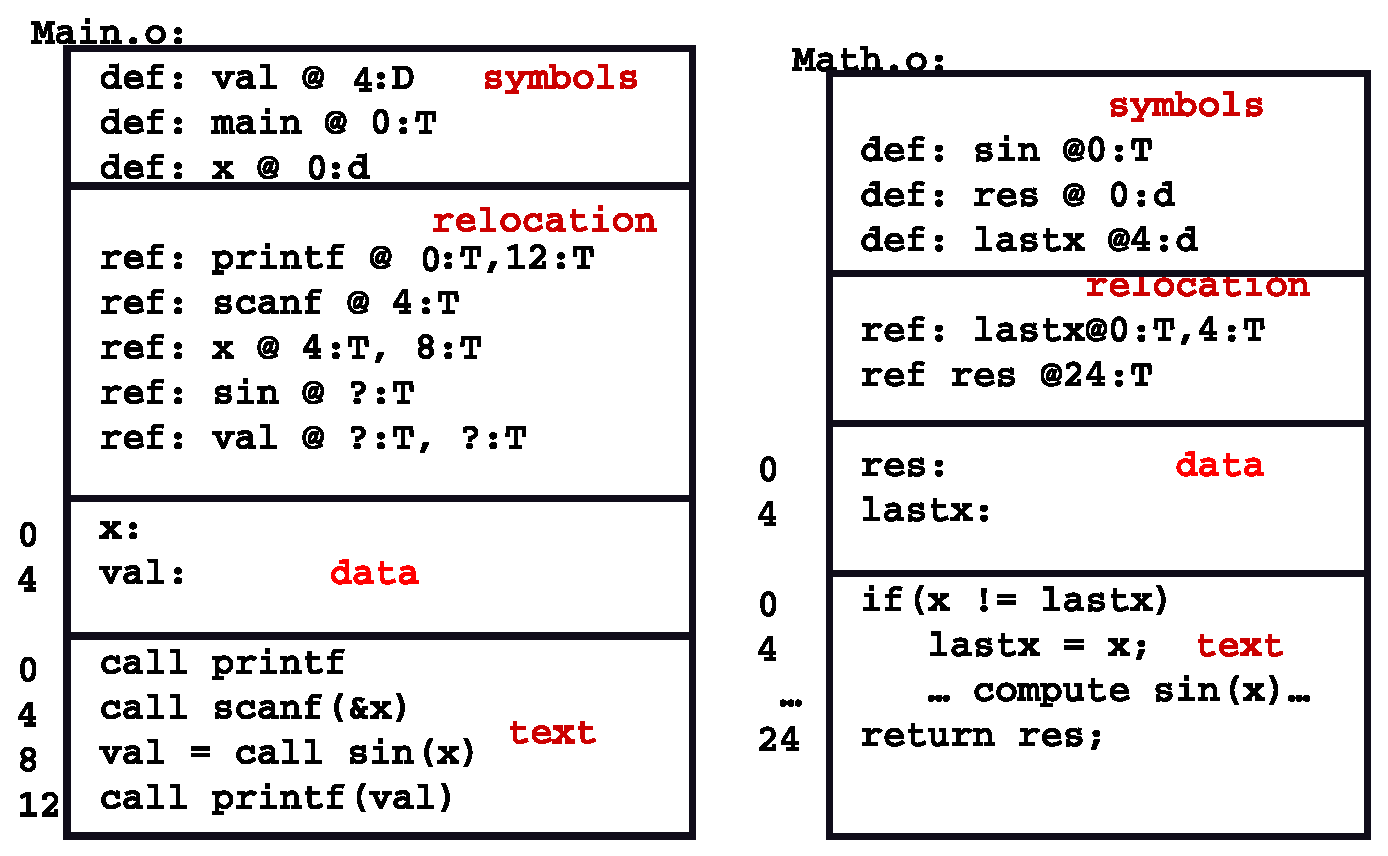
\includegraphics[width=4.8in]{figs/2mobj}}
\end{slide}

\begin{slide}{Passe 1: Réorganisation des segments}
\vspace*{-.2in}
\centerline{\includegraphics[width=4.8in]{figs/2mreorg}}
\end{slide}

\begin{slide}{Passe 2: Résolution des adresses}
\vspace*{-.2in}
\centerline{\includegraphics[width=4.8in]{figs/2mreloc}}
\end{slide}

%\begin{slide}{Écriture finale}
%\vspace*{-.2in}
%\centerline{\includegraphics[width=4.8in]{figs/2mout}}
%\end{slide}

\begin{slide}{Examiner les programmes avec nm}
\begin{columns}
\column{47mm}
\begin{block}{}
\begin{alltt}
int \Green{uninitialized};
int \Maroon{initialized} = 1;
const int \Blue{constant} = 2;
int main ()
\{
  return 0;
\}
\end{alltt}
\end{block}
\column{0mm}
\column{2.2in}
\large\ttfamily\obeylines%
\$ nm a.out
\ldots
\annotate[(label.south east) -- (text.north west)]{0400400}{-12mm,8mm}{VA} %
\annotate[(label.south west) -- (text.north east)]{T}{18mm,8mm}{symbol type} %
\_start
04005bc \Blue{R} constant
0601008 W data\_start
0601020 \Maroon{D} initialized
04004b8 T main
0601028 \Green{B} uninitialized
\end{columns}
\bigskip
\itms{
  \item \texttt{const} variables \Blue{\ttfamily R} en lecture seule
  \ittms{
    \item Choix d'une adresse \texttt{constant} sur la même page que \texttt{main}
    \item Partage de pages en lecture seule
  }
  \item Données à zéro dans le segment ``BSS'', \Green{\ttfamily B}
  \ittms{
    \item Pas de place réservée dans le .exe
    \item Des pages remplies de 0 sont allouées par le SE à la demande
  }
}
\end{slide}

\begin{slide}{Examiner des programmes avec objdump}
\vspace*{4mm}
{\openup-1.5mm
\begin{alltt}
\$ objdump -h a.out
a.out:     file format elf64-x86-64
Sections:
Idx Name    Size      VMA       \tikznode{lma}{LMA}       \tikznode{off}{File off}  Algn
\ldots
 12 .text   000001a8  00400400  00400400  00000400  2**4
            CONTENTS, ALLOC, LOAD, READONLY, CODE
\ldots
 14 .rodata 00000008  004005b8  004005b8  000005b8  2**2
            CONTENTS, ALLOC, LOAD, READONLY, DATA
\ldots
 17 .ctors  00000010  00600e18  00600e18  00000e18  2**3
            CONTENTS, ALLOC, LOAD, DATA
\ldots
 23 .data   0000001c  00601008  00601008  00001008  2**3
            CONTENTS, ALLOC, LOAD, DATA
\ldots
 24 .bss    0000000c  00601024  00601024  00001024  2**2
            ALLOC\tikznode{nocontents}{\strut}
\ldots
\end{alltt}}
\begin{tikzpicture}[overlay,remember
        picture,red,thick,<-,font=\sffamily]
\draw (nocontents.east)
  -- +(10mm,-2mm) node[anchor=west] {N'occupe pas de place dans le bin};
\draw (off) -- +(-10mm,+10mm) node[text width=80mm,anchor=south] (note)
      {LMA.\ et File off ont \\[-1mm]
          le même aligne:ment de page};
\draw (lma.north east) -- (note);
\end{tikzpicture}
\end{slide}

\begin{slide}{Types de résolution de liens}
\itms{
\item Patche avec une adresse absolue
\ittms{
  \item Exemple: \Red{\texttt{int y, *x = \&y;}} \\
  \item \Red{\texttt{call printf}} devient\\
    \Red{\texttt{8048248: e8 e3 09 00 00\quad call 8048c30 <printf>}}
  \item L'encodage binaire correspond à l'adresse virtuelle de \texttt{printf} \\
     (Attention: encodage de l'argument de \texttt{call} est relatif au PC)
}
\item Patche avec un offset
\ittms{
  \item Utilisé pour les structures
  \item Exemple: \texttt{struct queue \char`\{\ int type;
      void *head; \char`\}\ q;}\\
    \Red{\texttt{q.head = NULL}} $\to$ \Red{\texttt{movl \$0,
          q+4}} $\to$ \Red{\texttt{movl \$1, 0x804a01c}}
}
\item Ajouter la différence entre le segment original (dans le .o) et final.
}
\end{slide}

%\begin{slide}{Name mangling}
%\begin{columns}[b]
%\column{47mm}
%\begin{block}{}
%\openup-1\jot\ttfamily\obeylines\obeyspaces%
%// C++
%int \Red{foo} (int a)
%\{
%~ return 0;
%\}\\[\baselineskip]
%int \Purple{foo} (int a, int b)
%\{
%~ return 0;
%\}
%\end{block}
%\column{2.5in}
%\ttfamily\obeyspaces\obeylines%
%\% \Green{nm overload.o}
%0000000 T \Red{\_Z3fooi}
%000000e T \Purple{\_Z3fooii}
%~       U \tikznode{personality}{\_\_gxx\_personality\_v0} \\[3ex]
%\% \Green{nm overload.o | \annotate[(label.east)--(text.north west)]{c++filt}{-25mm,4mm}{Demangle names}}
%0000000 T \Red{foo}(int)
%000000e T \Purple{foo}(int, int)
%~       U~\_\_gxx\_personality\_v0
%\end{columns}
%\begin{tikzpicture}[overlay,remember
%        picture,red,thick,<-,font=\sffamily]
%\draw (personality) -- +(7mm,15mm) node[right=8mm,text width=40mm,anchor=south]
%    { Mangling not\\[-1mm] compatible across\\[-1mm] compiler versions };
%\end{tikzpicture}
%\itms{
%  \item C++ can have many functions with the same name
%  \item Compiler therefore \emph{mangles} symbols
%  \ittms{
%    \item Makes a unique name for each function
%    \item Also used for methods/namespaces
%      (\texttt{obj::fn}),  template
%      instantiations, \& special functions
%      such as \texttt{operator new}
%  }
%}
%\end{slide}

%\begin{slide}{Initialization and destruction}
%\vspace*{-2mm}
%\begin{columns}[T]
%\column{47mm}
%\vspace*{-1mm}
%\begin{block}{}
%\ttfamily\obeylines\obeyspaces%
%// C++
%int a\_foo\_exists;
%struct foo\_t \{
%~ \Red{foo\_t} () \{
%~   a\_foo\_exists = 1;
%~ \}
%\};
%foo\_t foo;
%\end{block}
%\column{2.7in}
%\itms{
%  \item Initializers run before main
%  \ittms{
%    \item Mechanism is platform-specific
%  }
%  \item Example implementation:
%  \ittms{
%    \item Compiler emits static function in each file running
%      initializers
%    \item Wrap linker with \texttt{collect2} program that generates
%      \texttt{\_\_\_main} function calling all such functions
%    \item Compiler inserts call to \texttt{\_\_\_main} when compiling
%      real \texttt{main}
%  }
%}
%\end{columns}
%\vspace*{-1mm}
%\openup-1.5\jot
%\begin{alltt}
%\% \Green{cc -S -o- ctor.C | c++filt}
%\ldots
%        .text
%        .align 2
%\_\_static\_initialization\_and\_destruction\_0(int, int):
%\ldots
%        call    \Red{foo_t::foo_t()}
%\end{alltt}
%\end{slide}
%
%\begin{slide}{Other information in executables}
%\begin{columns}
%\column{47mm}
%\begin{block}{}
%\ttfamily\obeylines\obeyspaces%
%// C++
%struct foo\_t \{
%~~\Red{\char`\~foo\_t}() \{/*...*/\}
%~~except() \{ throw 0; \}
%\};
%void fn ()
%\{
%~ foo\_t foo;
%~ foo.except();
%~ /* ... */
%\}
%\end{block}
%\column{2.7in}
%\itms{
%  \item Throwing exceptions destroys automatic variables
%  \item Must find all such variables
%  \ittms{
%    \item In all procedures' call frames until exception caught
%    \item All variables of types with non-trivial destructors
%  }
%  \item Record info in special sections
%}
%\end{columns}
%\itms{
%  \item Executables can include debug info (compile w.\ \texttt{-g})
%  \ittms{
%    \item What source line does each binary instruction correspond to?
%  }
%}
%\end{slide}

\begin{slide}{Variation 0: Linker dynamique}
\itms{
  \item Pourquoi ne pas linker à l'exécution ?
  \ittms{
    \item Si un code n'est pas trouvé, on va le chercher
    \item Chargement de code \emph{à la demande} \\
\centerline{\includegraphics[width=4.8in]{figs/dynamic}}

  \item Problèmes: Différences par rapport au Linker statique ?
  Où aller chercher le code manquant ? Que faire si résolution impossible ?
}
}
\end{slide}

\begin{slide}{Variation 1: Bibliothèque partagée statique}
\itms{
  \item Observation: la plus part des programmes utilisent la bibliothèque statique,
  libc.a.\\ Plein de copies inutiles.

  \centerline{\includegraphics[width=4in]{figs/ls-gcc}}
  \item Idée: une seule copie sur disque inclue dans chaque programme.}
\end{slide}

\begin{slide}{Bibliothèque partagée statique}
\hspace*{-4mm}\vbox{
\itms{
\item Définir un segment réservé à une adresse fixe dans l'espace d'adressage de chaque programme
}
\vspace*{-4ex}
\centerline{\includegraphics[width=3.5in]{figs/staticshared}}
%\vspace*{-2ex}
\hbox{\begin{minipage}{2.9in}
\ittms{
\item On alloue un morceau de ce segment à chaque bibliothèque partagée statique
}
\end{minipage}
\begin{minipage}{2in}
\includegraphics[width=2in]{figs/sslibs}
\end{minipage}}
\ittms{
\item Le loader marque la région comme invalide
\item Si le processus saute dans la région, le SE déclenche un seg fault, qui
  est récupéré par le loader qui peut charger le code depuis une zone mémoire
  partagée.
\item Plusieurs programmes se partagent le même code.
}}
\end{slide}

\begin{slide}{Variation 2: Bibliothèques partagées dynamiques}
\itms{
\item Inconvénient du statique: zone fixe pré-allouée dans tous les processus
\ittms{
  \item Espace perdu
  \item Et si la librairie dépasse la taille de la zone fixe ?
}
\item Solution: Chargement dynamique de bibliothèques partagées
\ittms{
  \item Chargement d'une librairie possible à n'importe quelle adresse
  \item Problème: le linker ne sait pas où le code sera chargé ...
}
}
\end{slide}

\begin{slide}{PIC: Code position-indépendant}
% PLT (procedure linkage table) slide, but PLT in figures
\hbox{
  \begin{minipage}{2.5in}
\itms{
  \item Le code de la bibliothèque doit pouvoir tourner indépendemment de l'adresse
  \item Ajouter un niveau d'indirection!
}
\includegraphics[width=2in]{figs/staticlib}
  \end{minipage}
  \begin{minipage}{2in}
\includegraphics[width=2in]{figs/dshlib}
  \end{minipage}
}
\end{slide}

\begin{slide}{Chargement à la demande}
\hbox{
  \begin{minipage}{2.2in}
\hspace*{-.2in}\includegraphics[width=5in]{figs/lazy}\hss
  \end{minipage}
  \begin{minipage}{2.5in}
\itms{
  \item Faire la résolution au chargement est coûteux
  \item Un programme n'utilise que quelques fonctions
  \item Résolution faite lors du premier appel
}
\vspace*{1.2in}
  \end{minipage}
}
\end{slide}

%\begin{frame}
%\frametitle{ELF}
%\begin{itemize}
%  \item Today many systems use ELF as a binary format
%  \item Every ELF file has an \emph{ELF header} (\texttt{readelf -h }
%    \emph{file})
%  \item Files ready to be run by OS have \emph{program headers}
%  \begin{itemize}
%    \item Examine with \texttt{readelf -l } \emph{file}
%    \item Goes near beginning of file; says where to load what and how
%  \end{itemize}
%  \item Files that need to be linked have \emph{section headers}
%  \begin{itemize}
%    \item Examine with \texttt{readelf -S } \emph{file}
%    \item Goes at end of file (may not need to be mapped in)
%  \end{itemize}
%\end{itemize}
%\end{frame}
%
%\begin{frame}
%\frametitle{Dynamic linking with ELF}
%\begin{itemize}
%  \item Every dynamically linked executable needs an
%    \emph{interpreter}
%  \begin{itemize}
%    \item Embedded as string in special \texttt{.interp} section
%    \item \texttt{readelf -p .interp /bin/ls} $\to$
%      \texttt{/lib64/ld-linux-x86-64.so.2}
%    \item So all the kernel has to do is run \texttt{ld-linux}
%  \end{itemize}
%  \item \texttt{dlfixup} uses hash table to find symbols when needed
%  \item Hash table lookups can be quite expensive
%      \href{http://www.akkadia.org/drepper/dsohowto.pdf}{[Drepper]}
%  \begin{itemize}
%    \item E.g., big programs like OpenOffice very slow to start
%    \item Solution 1:  Use a better hash function
%    \begin{itemize}
%      \item linux added \texttt{.gnu.hash} section, later removed
%        \texttt{.hash} sections
%    \end{itemize}
%    \item Solution 2:  Export fewer symbols (it is now fashionable to
%      use:
%    \begin{itemize}
%      \item \texttt{gcc -fvisibility=hidden} (keep symbols local to DSO)
%      \item \texttt{\#pragma GCC visibility
%          push(hidden)}/\texttt{visibility pop}
%      \item \texttt{\_\_attribute\_\_(visibility("default"))},
%        (override for a symbol)
%    \end{itemize}
%  \end{itemize}
%\end{itemize}
%\end{frame}
%
%\begin{slide}{Code = data, data = code}
%\itms{
%\item No inherent difference between code and data
%\ittms{
%  \item Code is just something that can be run through a CPU without
%    causing an ``illegal instruction fault''
%  \item Can be written/read at runtime just like data ``dynamically
%    generated code''
%}
%\item Why?  Speed (usually)
%\ittms{
%  \item Big use: eliminate interpretation overhead.  Gives 10-100x performance improvement
%  \item Example: Just-in-time compilers for java, or qemu vs.\ bochs.
%  \item In general: optimizations thrive on information.  More information at runtime.
%}
%\item The big tradeoff:
%\ittms{
%  \item Total runtime = code gen cost + cost of running code
%}
%}
%\end{slide}
%
%\begin{slide}{How?}
%\itms{
%\item Determine binary encoding of desired instructions \\[-2ex]
%\centerline{\includegraphics[width=4in]{figs/sparcsub}}
%\item Write these integer values into a memory buffer\\[-.5ex]
%\centerline{\includegraphics[width=4in]{figs/sparcsubgen}}
%\item Jump to the address of the buffer:\\
%  \texttt{((int (*)())code)();}
%}
%\end{slide}
%
%
%\begin{slide}{Linking and security}
%\begin{columns}[c,onlytextwidth]
%\column{31mm}
%\begin{block}{}
%\ttfamily\obeylines\obeyspaces%
%void fn ()
%\{
%~~char buf[80];
%~~gets (buf);
%~~/* ... */
%\}
%\end{block}
%\column{80mm}
%\begin{enumerate}
%  \item Attacker puts code in buf
%  \ittms{
%    \item Overwrites return address to jump to code
%  }
%  \item Attacker puts shell command above buf
%  \ittms{
%    \item Overwrites return address so function ``returns'' to
%      \texttt{system} function in libc
%  }
%\end{enumerate}
%\end{columns}
%\itms{
%  \item People try to address problem with linker
%  \item W\char`\^X: No memory both writable and executable
%
%  \ittms{
%    \item Prevents 1 but not 2, must be disabled for jits
%  }
%  \item Address space randomization
%  \ittms{
%    \item Makes attack \#2 a little harder, not impossible
%  }
%  \item Also address with compiler (stack protector)
%}
%\end{slide}
%
%\begin{frame}{Segments ELF != Segments Dynamiques}
%
%\begin{itemize}
%\itemsep1pt\parskip0pt\parsep0pt
%\item
%  Attention à ne pas confondre segments ELF et segments dynamiques
%\item
%  Démonstration interactive de:
%
%  \begin{itemize}
%  \itemsep1pt\parskip0pt\parsep0pt
%  \item
%    \texttt{objdump} et \texttt{readelf}
%  \item
%    \texttt{/proc/\textless{}pid\textgreater{}/maps}
%  \end{itemize}
%\end{itemize}
%\end{frame}



\begin{slide}{Résumé: Édition de Liens}
\vspace*{-.1in}
\itms{
\item Compilateur: 1 fichier objet par fichier source
\ittms{
  \item Problème: vue incomplète du monde
  \item Solution: utiliser des références symboliques (``\texttt{printf}'')
}
\item Linker: combine les .o dans un seul exécutable
\ittms{
  \item Vue globale
  \item Patche les références symboliques
  \item Interface avec le SE, où est le code ? les données ? où commence le
  programme ?
}
}
\end{slide}

\end{document}
